%%%%% Don't Make Changes Below Here %%%%%
\documentclass{article}\usepackage{listings}\usepackage[utf8]{inputenc}\usepackage[margin=0.4cm,top=0.4cm,bottom=0.4cm]{geometry}\usepackage[usenames,dvipsnames,svgnames,table]{xcolor}\usepackage{calligra}\usepackage{tikz}\usetikzlibrary{matrix,fit,chains,calc,scopes}\usepackage{tcolorbox}\tcbuselibrary{skins}\tcbset{Baystyle/.style={sharp corners,enhanced,boxrule=6pt,colframe=Green,height=\textheight,width=\textwidth,borderline={8pt}{-11pt}{},}}\usepackage{amsmath,amssymb,amsthm,tikz,tkz-graph,color,chngpage,soul,hyperref,csquotes,graphicx,floatrow}\newcommand*{\QEDB}{\hfill\ensuremath{\square}}\newtheorem*{prop}{Proposition}\renewcommand{\theenumi}{\alph{enumi}}\usepackage[shortlabels]{enumitem}\usetikzlibrary{matrix,calc}\MakeOuterQuote{"}\newtheorem{theorem}{Theorem} \usetikzlibrary{shapes} \usepackage{lipsum}\usepackage{tabularx,ragged2e,booktabs,caption}\tcbuselibrary{breakable}\newenvironment{yframed}{\begin{tcolorbox}[breakable,colback=gray!3,title after break={\textit{\color{red}Solution (cont.)}},colbacktitle=gray!3, coltitle=black,titlerule=-1pt] }{\end{tcolorbox}}\newtcolorbox{mybox}{colback=black!15!white, colframe=white,arc=12pt}\newtcolorbox{myboxot}{colback=green!15!white, colframe=white,arc=12pt}\newtcbox{\mylib}{enhanced,boxrule=0pt,top=0mm,bottom=0mm,right=0mm,left=4mm,arc=4pt,boxsep=9pt,before upper={\vphantom{dlg}},colframe=green!50!black,coltext=green!25!black,colback=green!10!white,overlay={\begin{tcbclipinterior}\fill[green!75!blue!50!white] (frame.south west)rectangle node[text=white,font=\sffamily\bfseries\tiny,rotate=90] {Problem} ([xshift=4mm]frame.north west);\end{tcbclipinterior}}}\newtcbox{\mylibot}{enhanced,boxrule=0pt,top=0mm,bottom=0mm,right=0mm,arc=4pt,boxsep=9pt,before upper={\vphantom{dlg}},colframe=green!50!black,coltext=green!25!black,colback=green!10!white,overlay={\begin{tcbclipinterior}\fill[red!75!blue!50!white] (frame.south west)rectangle node[text=white,font=\sffamily\bfseries\tiny,rotate=90] {Other} ([xshift=4mm]frame.north west);\end{tcbclipinterior}}}\usepackage{algorithm}\usepackage[noend]{algpseudocode}\makeatletter\def\BState{\State\hskip-\ALG@thistlm}\makeatother\def\T{\indent}\def\star{\bigstar}
\def\Title{\begin{tcolorbox}[Baystyle,]{\begin{center}\vspace*{0.14\textheight}
{\rule{\textwidth}{1.6pt}\vspace*{-\baselineskip}\vspace*{2pt}}

\rule{\textwidth}{0.4pt}\\[0.2\baselineskip]{\fontsize{45}{45}\scshape CS 170: Efficient Algorithms and \\[-0.3\baselineskip] Intractable Problems \\[0.2\baselineskip] \calligra Spring 2017 \\[0.2\baselineskip]}
{\rule{\textwidth}{0.4pt}\vspace*{-\baselineskip}\vspace{3.2pt}}

% change homework number here
\rule{\textwidth}{1.6pt}\\[\baselineskip]\vspace{0.05\textheight}{{\fontsize{45}{45}\scshape$\bullet$\\ {Homework 7}\\ 
% change due date here
\vspace*{0.01\textheight} }{{\fontsize{18}{18}\scshape{Due on April 4 at 12:00pm\\}}}\fontsize{45}{45}\scshape$\bullet$  \\}

\vspace*{0.1\textheight}{\fontsize{12}{12}\calligra Solutions by\\}{\fontsize{28}{28}\scshape \Name \\}\vspace*{0.01\textheight}{\fontsize{12}{12}\scshape \SID} \\\vspace*{0.05\textheight}{\fontsize{12}{12}\calligra In collaboration with\\}\vspace*{0.01\textheight}{\fontsize{12}{12}\scshape \Collabs} \\\vspace*{0.05\textheight}\end{center}}\end{tcolorbox}\newgeometry{margin=0.75in}}\def\BeginSolution{\begin{yframed}\textbf{\color{red}Solution }}\def\EndSolution{\end{yframed}}
%%%%% Don't Make Changes Above Here %%%%%
\usepackage{fancyvrb}
%%%%% Template Begins Here %%%%%

\def\Name{Ninh DO}  % Your name 
\def\SID{25949105}  % Your student ID number
\def\Collabs{None} % Your collaborators here with a comma between each person's name. Write None if no collaborators. Don't leave blank.


\pagestyle{empty}
\begin{document}
\Title

%%%% Problem 1 Starts Here %%%%
\vspace{1mm}\noindent\begin{mybox}{\begin{center}\textbf{\color{black}
% change problem name here
Problem 1: Linear Programming Fundamentals
}\end{center}}\end{mybox}\vspace{1mm}
% change difficulty level here
\begin{myboxot}\noindent\textbf{$\star$ Level}\end{myboxot} 
\noindent For each of the following optimization problems, is there a finite optimal solution that can be found by an LP solver? If the answer is no, identify the reason why (i.e. unbounded, infeasible, or not a linear program).
\begin{enumerate}[(a)]
	\item \[\text{max }5x+3y\]\begin{align*}
		x^2+y\le&45\\
		x\le&7\\
		x,y\ge&0
	\end{align*}
\BeginSolution % 1a
% Solution Here
\\
YES. Can be NO if we consider this problem non-LP as the first constraint is not linear. However, we can always modify the LP solver to solve this particular non-LP. 
\EndSolution
	\item \[\text{max }8x + \frac{1}{13}y+z\]\begin{align*}
		x\le&5\\
		4x+3z\le&9\\
		x,y,z\ge&0
	\end{align*}
\BeginSolution % 1b
% Solution Here
\\
NO. Unbounded y
\EndSolution
\pagebreak
	\item \[\text{max }3x+3y\]\begin{align*}
		5x-2y\ge&0\\
		2x\le&18\\
		x,y\ge&0
	\end{align*}
\BeginSolution % 1c
% Solution Here
\\
YES
\EndSolution
	\item \[\text{max }2x+2y\]\begin{align*}
		x+2y \le& 12\\
		x \le& 6\\
		x+y \ge& 10\\
		x,y \ge& 0
	\end{align*}
\BeginSolution % 1d
% Solution Here
\\
NO. Infeasible: $x+y$ is both less than or equal 9 and greater than or equal 10.
\EndSolution
	\item \[\text{max }2x-3y\]\begin{align*}
		3x+5y \ge & 13\\
		x \le & 4\\
		x,y \ge & 0
	\end{align*}
\BeginSolution % 1e
% Solution Here
\\
YES
\EndSolution
\end{enumerate}

%%%% Problem 1 Ends Here %%%%
\clearpage

%%%% Problem 2 Starts Here %%%%
\vspace{1mm}\noindent\begin{mybox}{\begin{center}\textbf{\color{black}
% change problem name here
Problem 2: Matches for tutoring
}\end{center}}\end{mybox}\vspace{1mm}
% change difficulty level here
\begin{myboxot}\noindent\textbf{$\star\star\star$ Level}\end{myboxot} 

\noindent A tutoring service has contracted you to work on pairing tutors with tutees. You are given a set of tutors $U$ and a set of tutees $V$. Everyone has filled out some questionnaires, so you know which tutors are compatible with which tutees (i.e. able to tutor the right subject). Additionally, each tutor i has given a limit $c_i$ on how many tutees they want to work with. Each tutee only gets one tutor. Describe an efficient algorithm for assigning tutors to tutees, such that as many tutees receive tutoring as possible. Give only the main idea.

\vspace{5pt}
\BeginSolution
\\
Represent the problem as a directed graph in which vertices are tutors and tutees and edges direct from tutors to tutees if they are compatible. We can see that there are only edges from the tutor set $U$ to the tutee set V, but no edge within $U$ or $V$. This is a bipartile matching problem.\\
Set up a vertex $S$ directing to all tutors $u_i$ with edges of capacities $c_i$, and set up a vertex $T$ to which all tutees $v_i$ direct with edges of capacities 1. The directed edges from tutors to tutees are assigned capacities 1.\\
Our algorithm is to run the maximum-flow algorithm from $S$ to $T$ for the above graph. To the end, the flow from $U$ to $V$ goes through the edges that match tutors to tutee satisfying the problem requirements.
\EndSolution

%%%% Problem 2 Ends Here %%%%
\clearpage

%%%% Problem 3 Starts Here %%%%
\vspace{1mm}\noindent\begin{mybox}{\begin{center}\textbf{\color{black}
% change problem name here
Problem 3: Criminal capture
}\end{center}}\end{mybox}\vspace{1mm}
% change difficulty level here
\begin{myboxot}\noindent\textbf{$\star\star\star\star$ Level}\end{myboxot} 
\noindent The Central Intelligence Agency has tasked you with preventing a criminal from fleeing the country. Roads and cities are represented as an unweighted directed graph $G = (V,E)$. We’re also given a set $C \subseteq V$ of possible current locations of the criminal, and a set $P \subseteq V$ of all airports out of the country. You want to set up roadblocks on a subset of the roads to prevent the criminal from escaping (i.e. reaching an airport).

\vspace*{5pt}
\noindent Clearly you could just put a roadblock at all the roads to each airport, but there might be a better way: for example, if the criminal is known to be at a particular intersection, you could just block all roads coming out of it. You may assume that roadblocks can be set up instantaneously.

\vspace*{5pt}
\noindent Give an efficient algorithm to find a way to stop the criminal using the least number of roadblocks.
\begin{enumerate}[(a)]
	\item Describe the main idea of your algorithm (no proof or pseudocode necessary).
	\BeginSolution % 3a
	\\
We set up a directed graph for the purpose of running maximum-flow algorithm: vertices are all cities and directed edges of capacity 1 are all roads. We consider two sets $C$ or $P$ for  a bipartile matching problem.\\
Set up a vertex $S$ directing to all criminals with edges of very large capacities, say infinity, and set up a vertex $T$ to which all out-of-the-country airports direct with edges of very large capacities, say infinity. The directed edges corresponding to roads are assigned capacities 1 as above.\\
Our algorithm is to run the maximum-flow algorithm from $S$ to $T$ for the above setting. To the end, the min-cut between $C$ and $P$ is the collection of roads on which we should put blocks.
	\EndSolution
	\item Analyze the asymptotic running time of your algorithm, in terms of $|C|, |P|, |V|, and |E|$.
	\BeginSolution % 3b
\\
The general runtime of maximum-flow problem is $O(\text{number of edges} * \text{maximum flow})$. The number of edges in our setting is $|C| + |P| + |E|$, the maxinum flow is $O(|E|)$. So the runtime is $O((|C| + |P| + |E|)*|E|)$. But $|C|, |P|$ are $O(|E|)$ since we do not consider isolated criminals or airports, so the total runtime can be said $O(|E|^2)$.
	\EndSolution
	\item Unfortunately we were too slow in implementing your roadblocks. The criminal has made it to an
	airport and is flying from city to city within the country. Your only option now is to shut down entire airports. Naturally, you want to minimize the number of airports you must shut down.
	
	\vspace*{5pt}
	We formulate this as a graph problem where $V$ is now the set of airports, and the (directed) edges $E$ represent flights from one airport to another. We still know a set $C \subseteq V$ of possible current locations of the criminal, and $P \subseteq V$ the set of all airports with flights leaving the country. Give an efficient algorithm to find the minimal set of airports (vertices) to block that will prevent the criminal from reaching $P$.
	\BeginSolution % 3c
\\
We duplicate every airport and set up a directed edge of capacity 1 between each pair of the identical airports.\\
The capacities of edge representing roads are 1. The capacities of edges from $S$ and edges to $T$ are infinity.\\
We run the maximum-flow algorithm from $S$ to $T$ for this setting, the min-cut going through the pair of the identical airports either in $C$ or $P$ give us the collection of airports that we should shut down.\\
The maximum flow is the number of vertices at most, so the runtime is $O((|C| + |P| + |E|)*|V|)$ or $O(|E|*|V|)$
	\EndSolution
\end{enumerate}

%%%% Problem 3 Ends Here %%%%
\clearpage

%%%% Problem 4 Starts Here %%%%
\vspace{1mm}\noindent\begin{mybox}{\begin{center}\textbf{\color{black}
% change problem name here
Problem 4: Another max flow algorithm
}\end{center}}\end{mybox}\vspace{1mm}
% change difficulty level here
\begin{myboxot}\noindent\textbf{$\star\star\star\star\star$ Level}\end{myboxot} 
\noindent Consider the following simple network with edge capacities as shown.

\begin{center}
	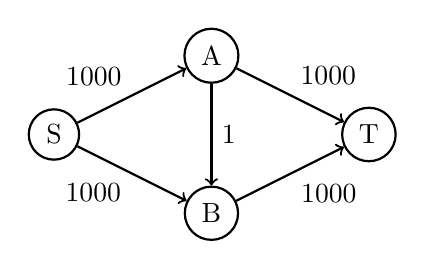
\begin{tikzpicture}[->,auto]
	\begin{scope}[every node/.style={circle,thick,draw}]
	\node (S) at (0,0) {S};
	\node (A) at (2,1) {A};
	\node (B) at (2,-1) {B};
	\node (T) at (4,0) {T};
	\end{scope}
	\begin{scope}[every edge/.style={draw,thick}]
	\path (S) edge node {$1000$} (A)
	          edge node[below,xshift=-14pt] {$1000$} (B)
		  (A) edge node {$1000$} (T)
		      edge node {$1$} (B)
		  (B) edge node[below,xshift=14pt] {$1000$} (T);
	
	\end{scope}
	\end{tikzpicture}
\end{center}

\begin{enumerate}[(a)]
\item Show that, if the Ford-Fulkerson algorithm is run on this graph, a careless choice of updates might cause it to take 2000 iterations. Imagine if the capacities were a million instead of 2000!
\BeginSolution
\\
Given the above graph, if we alternate between the paths $S-A-B-T$ and $S-B-A-T$, we will respectively decrease the capacities of $SA, BT$ and $SB, AT$ by 1 each time. The sum of two edges is 2000 so it needs 2000 iterations. 
\EndSolution

\item We will now find a strategy for choosing paths under which the algorithm is guaranteed to terminate
in a reasonable number of iterations. 

\vspace{5pt}
Consider an arbitrary directed network $(G = (V,E), s, t,\{c_e\})$ in which we want to find the maximum flow. Assume for simplicity that all edge capacities are at least 1, and define the capacity of an $s-t$ path to be the smallest capacity of its constituent edges. The fattest path from $s$ to $t$ is the path with the most capacity.

\vspace{5pt}
Show how to modify Dijkstra’s algorithm to compute the fattest $s-t$ path in a graph. The full four-part algorithm response is not needed, but provide a convincing justification that your modification finds this path.
\BeginSolution
\\
\underline{\textbf{Pseudocode:}}
%
\begin{lstlisting}
for all u in V:
	flow(u) = 0
	prev(u) = none
flow(s) = \infty
H = makequeue(V)     # (H is max heap using flow-values as keys)
while H is not empty:
	u = deletemax(H)
	for all edge (u,v) in E:
		if flow(v) < min(flow(u), c(u,v)):
			flow(v) = min(flow(u), c(u,v))    # c(u,v) is capacity of edge (u,v)
			prev(v) = u
			H.increasekey(v)
\end{lstlisting}
%
\underline{\textbf{Justification:}}\\
We use induction. If $v$ is one of the neighbors of source $s$, $flow(v) = min(flow(s), c(s,v)) = c(s,v)$ is exactly the fattest path from $s$ to $v$ since each path has only one edge. That is, the algorithm is correct up to at least one level away from s. We assume that the algorithm is correct up to $k$ levels away from $s$, which is $flow(u)$ is the fattest path from $s$ to $u$. We prove that the algorithm is correct up to the $k+1$ levels away from $s$, that is the neighbors of $u$: when $u$ is popped, the 'for' loop examines all the neighbors of $u$ and it will update the fasttest path up to that neighbor if it finds any alternative edge having the capacity larger than the previous capacity. This is done by the 'if' statement.\\
Since the algorithm examines all vertices, so it definitely reaches $t$ and update the fattest path from $s$ to $t$ along the way.
\EndSolution
\item Show that the maximum flow in $G$ is the sum of individual flows along at most $|E|$ paths from $s$ to $t$.
\BeginSolution
\\
This comes straightforward from the min-cut property. Consider the graph $G$ after we run the maximum-flow algorithm on it, let's look at a min-cut on this new $G$, the maximum flow is the sum of individual flows through edges on this min-cut, and the number of edges on this min-cut is equal to the number of paths from $s$ to $t$. The number of edges on this min-cut never exceeds $|E|$, so is the number of paths. Therefore, the above property holds.
\EndSolution
\item Now show that if we always increase flow along the fattest path in the residual graph, then the Ford-Fulkerson algorithm will terminate in at most $O(|E| \log F)$ iterations, where $F$ is the size of the maximum flow. (Hint: It might help to recall the proof for the greedy set cover algorithm in Section
5.4.)

\vspace{5pt}
In fact, an even simpler rule—finding a path in the residual graph using breadth-first search—guarantees
that at most $O(|V| \cdot |E|)$ iterations will be needed.
\BeginSolution
\\
Let $F_t$ be the maximum flow NOT obtained after t iterations (i.e. the remaining of the maximum flow), we have:
%
\begin{align*}
F_{t+1} \leq F_t - \frac{F_t}{|E|} = F_t\left(1-\frac{1}{|E|}\right)\\
F_t \leq F_0\left(1-\frac{1}{|E|}\right)^t < F_0\left(e^{-\frac{1}{|E|}}\right)^t = F * e^{-\frac{t}{|E|}}
\end{align*}
%
where $\frac{F_t}{|E|}$ is at least the amount of flow reduced after each iteration.\\
At $t = |E|\log F$, $F_t$ is strictly less than $F * e^{-\ln F} = 1$, or in other words the algorithm will terminate in at most $O(|E|\log F)$ iterations.
\EndSolution
\end{enumerate}

%%%% Problem 4 Ends Here %%%%
\clearpage


%%%% Problem 5 Starts Here %%%%
\vspace{-2mm}\noindent\begin{mybox}{\begin{center}\textbf{\color{black}
% change problem name here
Problem 5: Cannibal canisters
}\end{center}}\end{mybox}
\begin{myboxot}\noindent\textbf{$\star\star\star\star\star$ Level}\end{myboxot} 

\noindent You see n canisters, each with their own height $h_i$ and radius $r_i$ (they are perfectly cylindrical). A canister can eat another canister if it has a smaller height and radius. The eaten canister will be instantly consumed, and the eating canister will be tired for the rest of the day, unable to eat anymore. Design an algorithm to make as many canisters as possible get eaten (so they don’t try to eat you!) by the end of the day. Your solution should give the optimal order that canisters should eat each other, and the runtime should be $O(n^3)$. 

\vspace{5pt}
\noindent As an example, if there are three canisters with height and radius:
\begin{gather*}
	h_1 = r_1 = 1.5\\
	h_2 = r_2 = 2.5\\
	h_3 = r_3 = 3.5
\end{gather*}Then your output should be "$c_2$ eats $c_1$, $c_3$ eats $c_2$" or similar.
\begin{enumerate}[(a)]
	\item For this part, assume that $\forall i,h_i = r_i$. How would you solve the problem? Describe only the main idea and runtime, no need for pseudocode or proof.
\BeginSolution
\\
\underline{\textbf{Main idea:}}\\
Put all canisters in a min heap H with keys ordered by height or radius, then pop one by one out. The latter eats the former if it is strictly larger. If they are equal, put them in a queue to wait to be eaten. When a larger canister comes out, it will eat one in the queue in order. Say, if $a < b < c$, then $a$ popped out first, $b$ then popped out and eats $a$, $c$ then popped out and eats $b$. If $a = b = c < d < e < f$, then $a, b, c$ popped out and form a  queue, larger $d$ then popped out and eats $a$, x-larger $e$ then popped out and eats $b$, xx-larger $f$ then popped out and eats $c$. By this way, we can maximize the number of eaten canisters and resting canisters.\\
\underline{\textbf{Runtime:}}\\
$O(n \log n)$ to put all canisters into a min heap, $O(n)$ to pop them all. In general, the runtime is $O(n \log n)$
\EndSolution
	\item Solve the question fully, without the assumption that $h_i = r_i$. Hint: think about bipartite matching.
\BeginSolution
\\
\underline{\textbf{Main idea:}}\\
Step 1: Duplicate the set of canisters. That is, we work with two sets of the same canisters at the same time, say sets $U$ and $V$.\\
Step 2: Run two nested loops to construct a directed graph with edges of capacity 1 pointing from bigger canisters in $U$ to smaller canisters in $V$. The canister at edge tail must be strictly larger than, and thereby being able to eat, the canister at edge head in terms of height and radius.\\
Step 3: Set up the source $S$ pointing to each canisters in $U$ with edges of capacity 1.\\
Step 4: Set up the sink $T$ to which each canisters in $V$ points with edges of capacity 1.\\
Step 5: Run maximum-flow alrorithm for the setting above. At the cut between two sets, we have pairs of eating and eaten canisters, say (4,1), (2,3), (3,4), etc.\\
Step 6: Topologically sort these pairs, we end up with the food chain where the eating order start from the end. Say $2\rightarrow 3\rightarrow 4\rightarrow 1$ means: $4$ eats $1$, then $3$ eats $4$, then $2$ eats $3$.\\
\underline{\textbf{Runtime:}}\\
$O(n^2)$ to made egdes, $O(n^3)$ to run maximum-flow algorithm, $O(n)$ to topologically sort the canisters out. In general, the runtime is $O(n^3)$
\EndSolution
\end{enumerate}

%%%% Problem 5 Ends Here %%%%

\end{document}
%%%%% Template Ends Here %%%%%
